\section{Wigner Symbols}\label{sec:app.wignerSymbols}
Before discussing the Wigner symbols, we introduce the Clebsch-Gordan
coefficients as they appear quite naturally in the quantum theory
of angular momentum. Specifically, they are needed to study the coupling
of two systems having definite angular momenta. The material in this section
is inspired by \cite{VAR1988,BRI1993}. 

\subsection{Formal definitions}
\subsubsection{Clebsch-Gordan coefficients and Wigner $3j$-symbols}
Given two states that can be described by two quantum numbers
pertaining to their angular momenta, say $\ket{j_1m_1}$
and $\ket{j_2m_2}$ where $j_1$ and $j_2$ are the total
angular momenta and $m_1$ and $m_2$ are their $z$-projections. 
The states span two different vectors spaces, $\xi_1$ and $\xi_2$. 
To measure the angular momentum and associated $z$-projection
of the composite system, call them $j_3$ and $m_3$, we look at
the states spanning the product space $\xi_1\otimes\xi_2$. The product
states can be written
  \begin{equation}
   \ket{j_3m_3} = \sum_{m_1}\sum_{m_2}\ket{j_1m_1j_2m_2}\braket{j_1m_1j_2m_2|j_3m_3}
  \end{equation}
where
  \begin{equation*}
   \ket{j_1m_1j_2m_2}=\ket{j_1m_1}\otimes\ket{j_2m_2}
  \end{equation*}
and where the allowed values of $j_3$ and $m_3$ follow 
from the quantum vector addition rules. 

A similar relation holds for the bra. This equation simply 
describes the expansion of the a vector in the product space
$\xi_1\otimes\xi_2$ in the product of the bases of $\xi_1$ 
and $\xi_2$ \cite{COH1973b}. The expansion coefficients are known as the 
Clebsch-Gordan coefficients. Their square represent 
the probability that a measurement of the angular momentum 
yields a value of $\sqrt{j_3(j_3+1)}\hbar$.

We will note the Clebsch-Gordan coefficients
as
  \begin{equation}
    C^{j_3m_3}_{j_1m_1,j_2m_2} = \braket{j_1m_1j_2m_2|j_3m_3}.
  \end{equation}

We can now introduce the Wigner $3j$-symbols. They can be related
to the Clebsch-Gordan coefficients through
  \begin{equation}
   \begin{pmatrix} j_1 & j_2 & j_3 \\
		   m_1 & m_2 & m_3
   \end{pmatrix}
    = \frac{(-1)^{j_1-j_2-m_3}}{\sqrt{2j_3+1}}\braket{j_1m_1j_2m_2|j_3-m_3}.
  \end{equation}
More telling, though, is their interpretation as the probability
that three angular momenta couple to give zero angular momentum, or
  \begin{equation}
   \begin{pmatrix} j_1 & j_2 & j_3 \\
		   m_1 & m_2 & m_3
   \end{pmatrix}
    = (-1)^{j_1-j_2+j_3}\sum_{j'm'} C^{j'm'}_{j_1m_1,j_2m_2}C^{00}_{j'm',j_3m_3}.
  \end{equation}
The $3j$-symbols also appear in the angular integration of three spherical
harmonics 
  \begin{equation}
    \mathop{\iint}_\Omega Y_{j_1,m_1}(\theta,\varphi)Y_{j_2,m_2}(\theta,\varphi)Y_{j_3,m_3}(\theta,\varphi)d\Omega
      =
    \sqrt{\frac{(2j_1+1)(2j_2+1)(2j_3+1)}{4\pi}}\begin{pmatrix} j_1 & j_2 & j_3 \\ 0 & 0 & 0 \end{pmatrix}\begin{pmatrix} j_1 & j_2 & j_3 \\ m_1 & m_2 & m_3\end{pmatrix}
  \end{equation}

\subsubsection{Wigner $6j$-symbols}
The $6j$-symbols are related to the coupling of three angular momenta. In
this case, the resultant angular momentum $\bo{j}$ can be obtained via three 
different coupling schemes:
  \begin{enumerate}[I.]
   \item $\bo{j}_1+\bo{j_2}=\bo{j}_{12}, \qquad \bo{j}_{12}+\bo{j}_3=\bo{j}$;
   \item $\bo{j}_2+\bo{j_3}=\bo{j}_{23}, \qquad \bo{j}_1+\bo{j}_{23}=\bo{j}$;
   \item $\bo{j}_1+\bo{j_3}=\bo{j}_{13}, \qquad \bo{j}_{13}+\bo{j}_2=\bo{j}$.
  \end{enumerate}
Each coupling scheme has a set of associated \textit{generalized Clebsch-Gordan}
coefficients which gives the coefficients of the expansion of a state vector
in the basis of $\ket{j_1m_1,j_2m_2,j_3m_3}$. For instance, a state 
corresponding to coupling scheme I has expansion
  \begin{equation}
   \ket{j_1j_2(j_{12}),j_3jm} = \sum_{m_1,m_2,m_3}C_{j_{12}m_{12}j_3m_3}^{jm}C_{j_1m_1j_2m_2}^{j_{12}m_{12}}\ket{j_1m_1,j_2m_2,j_3m_3}
  \end{equation}
with similar expressions holding for the other coupling schemes.

We thus define the $6j$-symbols as the coefficients of the unitary
transformation that takes us from one scheme to another \cite{VAR1988}.
We can then write
  \begin{equation}
   \begin{Bmatrix} j_1 & j_2 & j_3 \\ j_4 & j_5 & j_6 \end{Bmatrix} = \frac{(-1)^{j_1+j_2+j_4+j_5}}{\sqrt{(2j_3+1)(2j_6+1)}}
      \sum_{m_1,m_2,m_3,m_4,m_6} C_{j_3m_3,j_4m_4}^{j_5m_5}C_{j_1m_1,j_2m_2}^{j_3m_3}C_{j_1m_1,j_6m_6}^{j_5m_5}C_{j_2m_2,j_4m_4}^{j_6m_6}
  \end{equation}


We can also define higher-order Wigner symbols, but things rapidly become complicated \cite{YUT1962}. 

\subsection{Numerical Computation of Wigner Symbols}
The previous section dealt with the definitions of 
the Clebsch-Gordan coefficients and the Wigner symbols. 
While more (much, much more) could have been said on the
subject, we will now discuss the actual evaluation of these
numbers. 

We note that the Condon-Shortley phase convention 
assures us all Clebsch-Gordan coefficients and 
Wigner symbols are real, which is a real numerical
advantage. 

Moreover, there exists closed-forms formulas in the form of algebraic
sums for the Wigner symbols, but they are riddled with numerical 
issues, such as the cancellation of large terms and the evaluation 
of the ratio of large factorial arguments. 

The best way to evaluate the coefficient was devised in 1975
by chemical physicist K. Schulten \cite{SCH1975}. 
He and R. G. Gordon 
rederived three-term recursion relation for the Wigner symbols 
and used them to evaluate sets of Wigner symbols at a time.
Fortran 
code exists\footnote{\url{http://cpc.cs.qub.ac.uk/summaries/ACWQ_v1_0.html}}, 
but our tests showed only \texttt{single} numerical precision. We have
thus reprogrammed the algorithm, first described in \cite{SCH1975}
and detailed in \cite{SCH1976}, in C++. 

Before detailing our results, we will briefly overview
the algorithm used (\see Figure \ref{fig:app.wigner.flowchart}. We compute
  \begin{align*}
    \begin{pmatrix}j_1 & j_2 & j_3 \\ m_1 & m_2 & m_3 \end{pmatrix} \qquad \forall j_1 \\
    \begin{Bmatrix}j_1 & j_2 & j_3 \\ j_4 & j_5 & j_6 \end{Bmatrix} \qquad \forall j_1
  \end{align*}
We can write the recursion relations valid for both symbols as 
(we adopt the notation of \cite{LUS1998})
  \begin{equation}
    \alpha_\psi(j_1)\psi(j_1+1)+\beta_\psi(j_1)\psi(j_1)+\gamma_\psi(j_1)\psi(j_1-1)=0
  \end{equation}
where $\psi(j_1)$ represents either the $3j$- or $6j$-symbol at $j_1$
and the Greek letters are the coefficient at that $j_1$. They are
shown in Table \ref{tab:app.wigner.coeffsRecursion}. 

To start the recursion, we would usually need two initial
conditions. It turns out, however, that the recursion
relations reduce to only two terms at the boundaries
$j_{1\text{min}}$ and $j_{1\text{max}}$. Like all
other numerical schemes, recursion relations
are only stable in the direction of increasing
coupling coefficients. Semi-classical analysis
\cite{SCH1975} informs us that there generally exists
three regions of interest for the function $\psi(j_1)$.
Near the boundaries, we are in the nonclassical 
regions. At the lower values of $j_1$, $\psi(j_1)$
is increasing until it hits the central classical
region, where it starts oscillating. On the other
hand, near the $j_{1\text{max}}$ boundaries, the
coefficients are increasing with decreasing $j_1$. 
Given the linearity of the recursion relations, we
can start the recursion relations from both boundaries
using a sufficiently small but otherwise \textit{arbitrary} number. 
While the ratios between successive values of the coupling coefficients
will be correct, their absolute values will not. The forward and backward
recurrences will be multiplied by a scalar, call them $c_1$ for the forward
recursion and $d_1$ for the backward recursion. To find the relationship
between the scalars, we watch the values of the forward and backward
recursions at some intermediary point. For more numerical stability, 
we use three contiguous values around the intermediary point
and find the parameter $\lambda=\nicefrac{d_1}{c_1}$ from a least-squares fit.
To choose the intermediary point, we note that the recursion relations
appear in the form
  \begin{equation}
   \psi(j_1+1)=X(j_1)\psi(j_1)+Y(j_1)\psi(j_1-1).
  \end{equation}
Schulten found that, using semiclassical analysis, 
that $|X(j_1)|$ attains its minimum value 
in the classical domain. Monitoring the variation
of $|X(j_1)|$ thus provides a way to find the intermediary point.

The overall scaling factor $c_1$ is found and the set of 
coupling coefficients is rescaled to its proper value
by using the normalization condition on the computed set.

We note that if the total size of the set is 1 ($j_{1\text{min}}=j_{1\text{max}}$), 
we can deduce, from the triangular condition, that $l_2\lor l_3=0$. We thus have
to evaluate the $3j$-symbols 
  \begin{align*}
   \begin{pmatrix} l_3 & 0 & l_3 \\ -m_3 & 0 & m_3 \end{pmatrix} &= \begin{pmatrix} l_3 & l_3 & 0 \\ m_3 & -m_3 & 0\end{pmatrix}=\frac{(-1)^{l_3-m_3}}{\sqrt{2l_3+1}}	\\
   \begin{pmatrix} l_2 & l_2 & 0 \\ -m_2 & m_2 & 0 \end{pmatrix} &= (-1)^{-2l_2}\begin{pmatrix} l_2 & l_2 & 0 \\ m_2 & -m_2 & 0\end{pmatrix}\\&=\frac{(-1)^{-l_2-m_3}}{\sqrt{2l_2+1}}
  \end{align*}
When the size is 2, we simply the two-term recursion formula with an arbitrary 
initial condition and normalize the two coefficients obtained. 

\begin{figure}
 \centering
 \begin{subfigure}[b]{0.5\textwidth}
  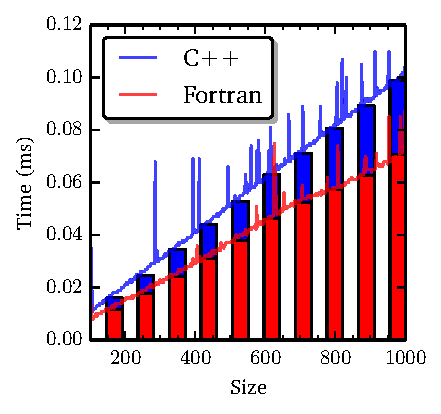
\includegraphics[width=\textwidth]{figs/backmatter/wignerTimes.pdf}
  \caption{Time (in ms) to compute sets of a given size of coupling coefficients, specifically the 
	    $3j$-symbol, in this case.}
 \end{subfigure}\hfill
 \begin{subfigure}[b]{0.5\textwidth}
  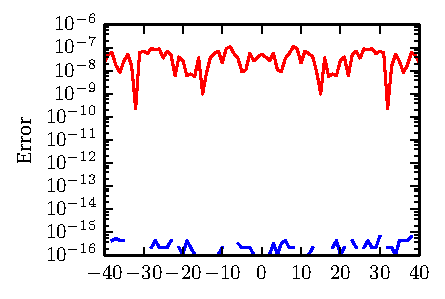
\includegraphics[width=\textwidth]{figs/backmatter/wignerPrecision.pdf}
  \caption{Precision of the Fortran and C++ implementations of the algorithm obtained%
	    by computing the orthogonality relationship \eqref{eq:app.wigner.orthogonality}.}
 \end{subfigure}
 \caption{Performance and precision of our numerical algorithms.}
\end{figure}

\begin{equation}
 \label{eq:app.wigner.orthogonality}
 \sum_{m1,m2} (2l_3+1)\begin{pmatrix} l_1 & l_2 & l_3 \\ m_1 & m_2 & m_3\end{pmatrix}^2=1
\end{equation}


\begin{table}
 \begin{center}
 \newcommand{\A}{$\begin{aligned}A(j_1) &=\left[j_1^2-(j_2-j_3)^2\right]^{1/2}\\&\phantom{=}\times\left[(j_2+j_3+1)^2-j_1^2\right]^{1/2}\\&\phantom{=}\times\left[j_1^2-m_1^2\right]^{1/2}\end{aligned}$}
 \newcommand{\B}{$\begin{aligned}B(j_1) &=-(2j_1+1)\\&\phantom{=}\times\left[j_2(j_2+1)m_1\right.\\&\phantom{=\times}-j_3(j_3+1)m_1\\&\phantom{=\times}\left.-j_1(j_1+1)(m_3-m_2)\right]\end{aligned}$}
 \newcommand{\E}{$\begin{aligned}E(j_1) &=\left\{\left[j_1^2-(j_2-j_3)^2\right]\right.\\&\phantom{=}\times\left[(j_2+j_3+1)^2-j_1^2\right]\\&\phantom{=}\times\left[j_1^2-(j_5-j_6)^2\right]\\&\phantom{=}\times\left.\left[(j_5+j_6+1)^2-j_1^2\right]\right\}^{1/2}\end{aligned}$}
 \newcommand{\F}{$\begin{aligned}F(j_1) &= (2j_1+1)\\&\phantom{=}\times\left\{j_1(j_1+1)\left[--+\right]\right.\\&\phantom{=\times}+j_5(j_5+1)\left[++-\right]\\&\phantom{=\times}+j_6(j_6+1)\left[+-+\right]\\&\phantom{=\times}\left.-2j_1(j_1+1)l_1(l_1+1)\right\}\end{aligned}$}
 \caption[Parameters and coefficients of the three-term recursion relations satisfied
	  by the $3j$- and $6j$-symbols.]
	 {Parameters and coefficients of the three-term recursion relations satisfied
	  by the $3j$- and $6j$-symbols.
	  The expression $[++-]$ represents the coefficient $[j_1(j_1+1)+j_2(j_2+1)-j_3(j_3+1)]$ and similarly for other signs in the bracket.}
 \label{tab:app.wigner.coeffsRecursion}
  \begin{tabular*}{\columnwidth}{m{0.1\textwidth}@{\extracolsep{\fill}}l@{\extracolsep{\fill}}l}
  \hline\hline
  $3j$- or $6j$-symbols	&	 $f(j_1)=\begin{pmatrix} j_1 & j_2 & j_3 \\ m_1 & m_2 & m_3 \end{pmatrix}$ & $h(j_1)=\begin{Bmatrix} j_1 & j_2 & j_3 \\ j_4 & j_5 & j_6 \end{Bmatrix}$\\
  \hline
  $\alpha_\psi$			& $j_1A(j_1+1)$		& $jE(j_1+1)$	\\
  $\beta_\psi$			& $B(j_1)$		& $F(j)$	\\
  $\gamma_\psi$			& $(j_1+1)A(j_1)$	& $(j_1+1)E(j)$	\\
				&			&		\\
  \multirow{4}{*}{Functions}	& \A			& \E		\\
  				&			&		\\
				& \B			& \F		\\
				&			&		\\
 \multirow{2}{*}{Endpoints}	& $j_{1\text{min}}=\text{max}(|j_2-j_3|,|m_1|)$ & $j_{1\text{min}}=\text{max}(|j_2-j_3|,|j_5-j_6|)$	\\
				& $j_{1\text{max}}=j_2+j_3$ 			& $j_{1\text{max}}=\text{min}(j_2+j_3,j_5+j_6)$		\\
				&			&		\\
 Normalization			& $\sum_{j_1}(2j_1+1)f(j_1)^2=1$		& $(2j_4+1)\sum_{j_1}(2j_1+1)h(j_1)^2=1$		\\
 				&			&		\\
 Sign				& $\text{sgn}[f(j_{1\text{max}})]=(-1)^{j_2-j_3-m_1}$ & $\text{sgn}[h(j_{1\text{max}})]=(-1)^{j_2+j_3+j_5+j_6}$\\
  \hline\hline
 \end{tabular*}
 \end{center}
\end{table}


% -- We draw a flowchart of the algorithm. 
% Block styles
\tikzstyle{decision} = [diamond, draw, fill=blue!20,text width=4.5em, text badly centered, node distance=3cm, inner sep=0pt]
\tikzstyle{block} = [rectangle, draw, fill=blue!20, text width=5em, text centered, rounded corners, minimum height=4em]
\tikzstyle{line} = [draw, -latex']
\tikzstyle{cloud} = [draw, ellipse,fill=red!20, node distance=3cm,minimum height=2em]
\tikzstyle{empty} = [fill=white]

% Actual flowchart
\begin{figure}
\begin{center}
\begin{tikzpicture}[scale=0.75,node distance = 2.8cm, auto]
 % -- We place the nodes
 \node [block] (init) {Enforce selection rules};
 \node [decision, below of=init] (sizeSets) {Determine boundaries and size of set};
 \node [block, below of=sizeSets] (size2) {Two-term forward recursion};
 \node [block, left of=size2] (size1) {Use analytical formula};
 \node [block, right of=size2] (otherSize) {Forward recursion};
 \node [decision,below of=otherSize] (overflow){$|\psi(j_1)|>$\\SRHUGE?};
 \node [block, left of=overflow](rescale) {Rescale forward recursion};
 \node [decision,below of=overflow] (monitor) {$|X(j_1)|$ increasing?};
 \node [decision,below of=monitor] (loopDone) {Loop done?};
 \node [block,left of=loopDone] (backward) {Backward recursion until midpoint};
 \node [block,below of=backward] (lambda) {Compute $\lambda$; rescale forward recursion};
 \node [block,right of=lambda] (normalization) {Normalize set of coefficients};
 \node [block, below of=normalization] (return){Return};
 
 % -- We place the edges
 \path [line] (init) -- (sizeSets);
 \path [line] (sizeSets) -| node [near end] {size$=1$} (size1);
 \path [line] (sizeSets) -- node [near start] {size$=2$} (size2);
 \path [line] (sizeSets) -| node [near end] {other sizes} (otherSize);
 \path [line] (otherSize) -- (overflow);
 \path [line] (overflow) -- node[near start]{yes} (rescale);
 \path [line] (overflow) -- node[near start]{no}  (monitor);
 \path [line] (rescale) |- (monitor);
 \path [line] (monitor.south west) -- node[near start]{yes} (backward.north east);
 \path [line] (monitor) -- node[near start]{no} (loopDone);
 \path [line] (loopDone.east) -- node[near start]{no} ($(loopDone.east)+(2,0)$) |- (otherSize.east);
 \path [line] (loopDone) -- node[near start]{yes} (normalization);
 \path [line] (normalization) -- (return);
 \path [line] (backward) -- (lambda);
 \path [line] (lambda) -- (normalization);
 \path [line] (size1) |- (return);
 \path [line] (size2.south) -- ($(size2.south)-(0,1)$) -- ++(-2,0) -- ($(lambda.south)-(2,1)$) -- ++(3,0) -- (normalization.south west);
\end{tikzpicture}
\end{center}
\caption[Flowchart of the algorithm used to compute the Wigner $3j$- and $6j$-symbols and Clebsch-Gordan coefficients.]
	{Flowchart of the algorithm used to compute the coupling coefficients. SRHUGE is the 
	  square root of the biggest representable number in our floating point representation.}
\label{fig:app.wigner.flowchart}
\end{figure}